% Generated by mdrender from preprint.md (theme: preprint). Compile with pdflatex.
\documentclass[10pt,letterpaper]{article}

\usepackage[T1]{fontenc}
\usepackage{lmodern}
\usepackage[spanish,es-nodecimaldot,es-noindentfirst,es-nosectiondot,es-tabla]{babel}
\usepackage[top=30mm,bottom=28mm,left=32mm,right=32mm]{geometry}
\usepackage{amsmath,amssymb}
\usepackage{graphicx}
\usepackage{booktabs}
\usepackage{fancyhdr}
\usepackage[hyphens]{url}
\usepackage{hyperref}
\hypersetup{
  colorlinks=true,
  allcolors=[rgb]{0.10,0.25,0.60},
  pdftitle={Cinética de conversión catalítica a baja temperatura},
  pdfauthor={Ana Pérez, Luis Gómez, Marta Ruiz},
  pdfkeywords={catálisis heterogénea, cinética, modelos de primer orden},
}

% Running head from page 2, folio centred at the foot (as the preprint theme prints them).
\pagestyle{fancy}
\fancyhf{}
\fancyhead[R]{\footnotesize\MakeUppercase{Preprint — 22 de noviembre de 2026}}
\fancyfoot[C]{\thepage}
\renewcommand{\headrulewidth}{0pt}

\title{Cinética de conversión catalítica a baja temperatura}
\author{%
  Ana Pérez\textsuperscript{1}, Luis Gómez\textsuperscript{1,2}, Marta Ruiz\textsuperscript{2}\\[1ex]
  {\small\itshape \textsuperscript{1}Departamento de Química, Universidad de Ejemplo, Santiago, Chile. ana.perez@ejemplo.org}\\
  {\small\itshape \textsuperscript{2}Instituto de Materiales Avanzados, Valparaíso, Chile.}%
}
\date{22 de noviembre de 2026}

\begin{document}

\maketitle
\thispagestyle{plain}

\begin{abstract}
Medimos la conversión de un sustrato modelo con dos catalizadores heterogéneos entre 20 y
60~°C. Ambos siguen una cinética de primer orden, pero el catalizador A alcanza el 90~\% de
conversión en menos de la mitad del tiempo que el B. Un modelo de dos parámetros reproduce
todas las curvas con un error menor al 2~\%, lo que permite elegir el catalizador según la
ventana de operación.

\medskip
\noindent\textbf{\textit{Palabras clave:}} catálisis heterogénea, cinética, modelos de primer orden
\end{abstract}

\section{Introducción}

La conversión catalítica a baja temperatura es clave para procesos que no toleran calor, como
la síntesis de compuestos sensibles o el tratamiento de efluentes [1, 2]. Elegir un catalizador
suele requerir largas campañas de ensayo; un modelo cinético simple acorta ese camino y permite
comparar candidatos con pocos experimentos\footnote{Los datos y el código del ajuste están
disponibles a pedido.}.

En este trabajo comparamos dos catalizadores comerciales y mostramos que un modelo de primer
orden, con una constante de velocidad que sigue la ley de Arrhenius, basta para describir la
conversión en todo el rango estudiado. Esto contrasta con trabajos anteriores que proponían
modelos de orden fraccionario para sistemas parecidos [3].

\section{Modelo cinético}

\subsection{Conversión en el tiempo}

Suponemos que la velocidad de conversión es proporcional a la fracción de sustrato que aún no
reacciona. Integrando, la fracción convertida $X(t)$ resulta
\begin{equation}
X(t) = X_\infty \left(1 - e^{-k t}\right),
\end{equation}
donde $X_\infty$ es la conversión final y $k$ la constante de velocidad.

\subsection{Dependencia con la temperatura}

La constante de velocidad sigue la ley de Arrhenius,
\begin{equation}
k(T) = A\, e^{-E_a / R T},
\end{equation}
de modo que dos mediciones a temperaturas distintas bastan para estimar la energía de
activación $E_a$:
\begin{equation}
E_a = \frac{R \ln (k_2 / k_1)}{1/T_1 - 1/T_2}.
\end{equation}

\section{Resultados}

La fracción convertida crece de forma monótona con el tiempo y se aproxima a uno para ambos
catalizadores (Figura 1). El catalizador A es claramente más rápido: llega al 50~\% de
conversión en 1,5~h, frente a 3,1~h del B.

\begin{figure}[htbp]
  \centering
  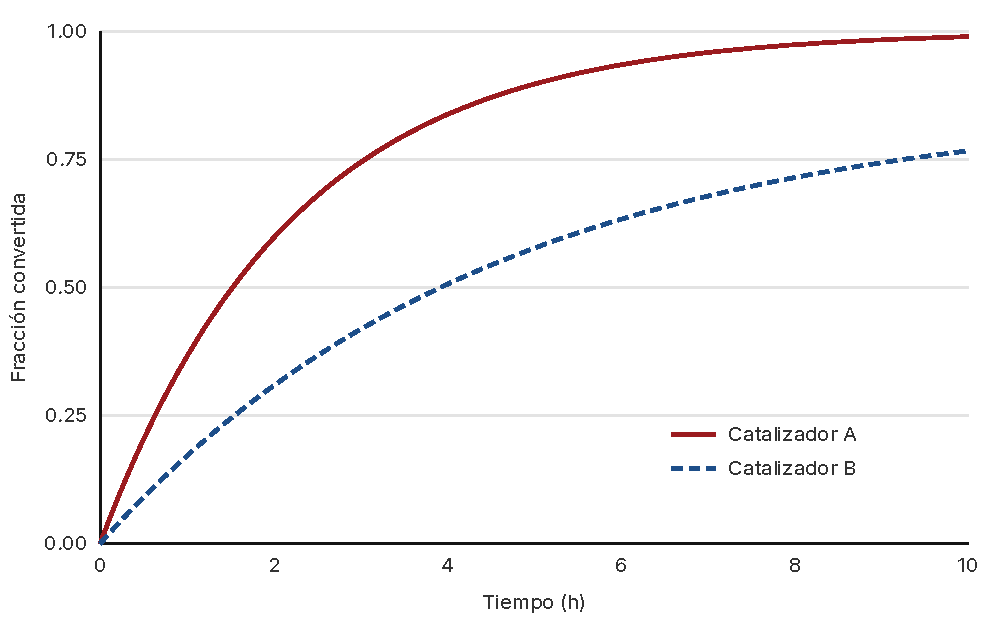
\includegraphics[width=0.85\linewidth]{figures/curva.pdf}
  \caption{Conversión en función del tiempo a 40~°C. La línea continua corresponde al
    catalizador A y la discontinua al B; cada curva es el promedio de tres ensayos.}
\end{figure}

Los parámetros ajustados con la ecuación (1) aparecen en la Tabla 1. La menor energía de
activación del catalizador A explica su ventaja, que además crece al bajar la temperatura.

\begin{table}[htbp]
  \centering
  \caption{Parámetros del modelo ajustados para cada catalizador.}
  \begin{tabular}{lrrrr}
    \toprule
    Catalizador & $X_\infty$ & $k$ a 40~°C (h$^{-1}$) & $E_a$ (kJ/mol) & $R^2$ \\
    \midrule
    A & 1,00 & 0,45 & 38,2 & 0,998 \\
    B & 0,86 & 0,22 & 44,7 & 0,995 \\
    \bottomrule
  \end{tabular}
\end{table}

\section{Discusión}

El modelo de primer orden describe bien ambos sistemas, sin necesidad de términos adicionales.
La diferencia en $X_\infty$ indica que el mecanismo de desactivación, y no solo la velocidad,
debe considerarse al elegir un catalizador [2].

\section{Conclusiones}

Un modelo de dos parámetros reproduce la conversión de ambos catalizadores con un error menor
al 2~\%. Para procesos continuos conviene el catalizador A; para operaciones por lotes cortas,
la diferencia es menor y el costo puede decidir.

\begin{thebibliography}{9}
\bibitem{ref1} Autor A, Autor B. Título de un artículo citado como ejemplo. Revista de Ejemplo. 2024;12(3):45--56.
\bibitem{ref2} Autor C. Título de un libro de ejemplo. 2.ª ed. Ciudad: Editorial de Ejemplo; 2023.
\bibitem{ref3} Autor D, Autor E, Autor F. Otro artículo citado como ejemplo. Revista de Ejemplo. 2022;10(1):1--12.
\end{thebibliography}

\end{document}
